%!TEX root = ../head.tex

\chapter{Übung}
\section{Einführung}
\subsection{}
\begin{enumerate}
	\item Datenformat inflexibel:
	\begin{enumerate}
		\item keine stand. Pfade
		\item viele Dateisys. erlauben keine Dateien über fixe Größe
		\item keine stand. Datentypen (.txt) und Schema der Datenspericherung leicht uneinheitl.
	\end{enumerate}
	\item mehrere Personen sollen/können darauf zugreifen
	\item Datenformat Abfragesprache/-tool auch neu "lernen" SQL einheitl.
	\item Redundanz sorgt für Anomalien (z.B. Aktualisierung d. Daten)
\end{enumerate}
\subsection{}
Rechteck: Entität, Raute: Bezeichner, Kreis: Attribute
\begin{enumerate}
	\item 3
	\item partielle Beziehungen
	\begin{itemize}
		\item SxT\(\to\)Ü
		\item ÜxT\(\to\)S
		\item SxÜ\(\to\)T
	\end{itemize}
	\item
	\begin{enumerate}
		\item Ein Tutor und ein Student nehmen an einer Übung teil
		\item An einer Übung mit einem Tutor nimmt ein Student teil
		\item Ein Student in einer Übung hat einen Tutor
	\end{enumerate}
	\item (1) und (3)
\end{enumerate}
\subsection{}
\begin{displaymath}
	A:N, C:M, B:1
\end{displaymath}
Faustregel: Auf der rechten Seite steht eine 1.
\subsection{}
ACHTUNG: Multiplizitäten genau andersrum wie bei 1.3
\begin{itemize}
	\item T:(1,*)
	\item Ü:(1,*)
	\item S:(0,1)
\end{itemize}
\subsection{}
\begin{itemize}
	\item Bahnhöfe M \(\leftrightarrow\) 1 Städte
	\item Bahnhöfe 1 \(\leftrightarrow\)verbindet\(\leftrightarrow\) 1 Bahnhöfe
	\item Bahnhöfe 1 \(\leftrightarrow\)verbindet\(\leftrightarrow\) N Züge
	\item Bahnhöfe 1 \(\leftrightarrow\)Start\(\leftrightarrow\) L Züge
	\item Bahnhöfe 1 \(\leftrightarrow\)Ziel\(\leftrightarrow\) K Züge
\end{itemize}

\section{ER-Modellierung}
\subsection{Prof-Stud}
\ref{img:Prof-Stud-ER}
\begin{figure}
	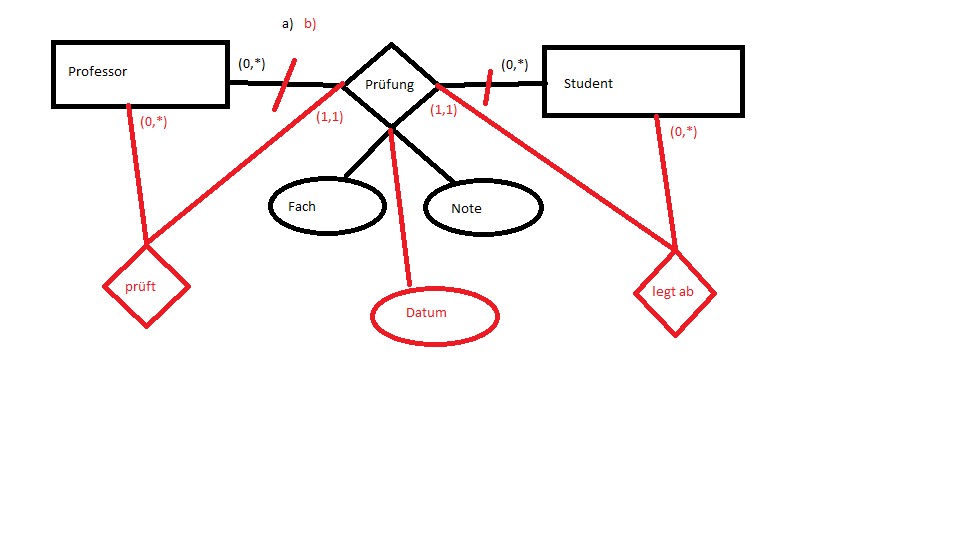
\includegraphics[width = 16cm]{./Database/Images/2_1.png}
	\caption{Professor-Student ER}
	\label{img:Prof-Stud-ER}
\end{figure}

\subsection{ER-Bahn}
\ref{img:Bahn-ER}
\begin{figure}
	\centering
	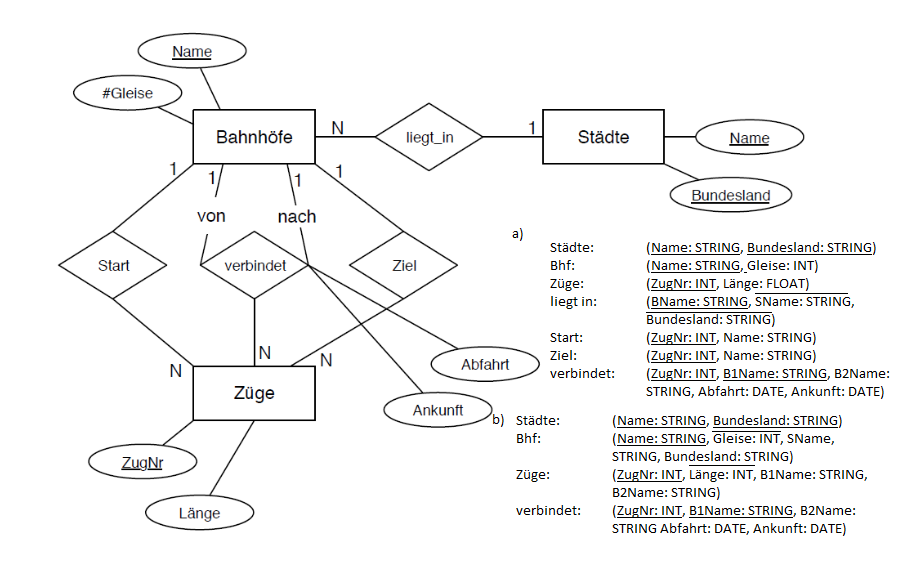
\includegraphics[width = 16cm]{./Database/Images/2_2.png}
	\caption{Bahnnetz ER}
	\label{img:Bahn-ER}
\end{figure}
\subsection{ER-Bsp}
\ref{img:Relations-ER}
\begin{figure}
	\centering
	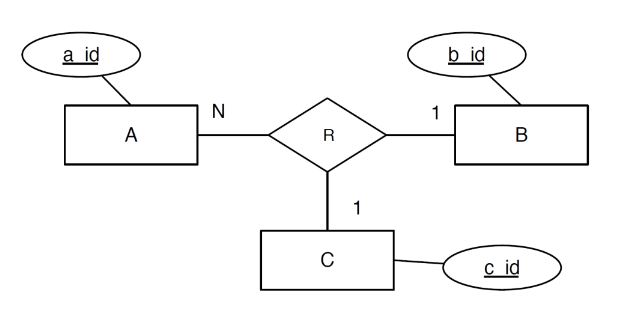
\includegraphics[width = 16cm]{./Database/Images/2_3a.png}
	\caption{Relations ER}
	\label{img:Relations-ER}
\end{figure}
\begin{enumerate}
	\item
	\begin{itemize}
		\item A x B \(\to\) C
		\item A x C \(\to\) B
	\end{itemize}
	\item
	\begin{itemize}
		\item A: (\underline{a id: INT})
		\item B: (\underline{b id: INT})
		\item C: (\underline{c id: INT})
	\end{itemize}
	\item
	\begin{itemize}
		\item \(R_1\): (\underline{a id}, \underline{b id}, c id)
		\item \(R_2\): (\underline{a id}, b id, \underline{c id})
	\end{itemize}
\end{enumerate}
\subsection{Vererbungshierarchie - Relationsschema }
\ref{img:Vererbungshierarchie}
\begin{figure}
	\centering
	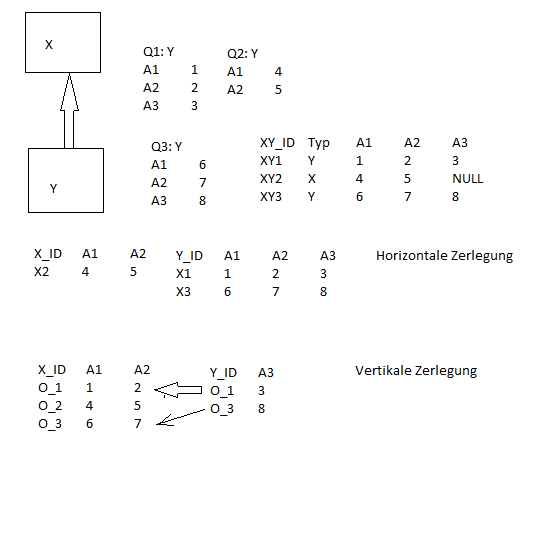
\includegraphics[width = 16cm]{./Database/Images/2_4.png}
	\caption{Relations ER}
	\label{img:Vererbungshierarchie}
\end{figure}

\section{Relationenalgebra}
dennis.koppenhagen@tu-dresden.de \\
\(\Pi\to\) Projektion, Spalte\\
\(\sigma\to\) Selektion, Zeile\\
\(\rho\to\) Umbenennung,\\
\subsection{}
\begin{enumerate}
	\item Geben Sie alle Vorlesungen an, die der Student X. gehört hat \\
	 \(R = \Pi_{\text{Titel, Vorl.Nr.}}\)(Vorlesung {\tiny \textifsym{|><|}} (hören {\tiny \textifsym{|><|}} \(\sigma_{\text{Name = X}}(\text{Studenten})\)))
	 \item Geben Sie die Titel der direkten Voraussetzungen für die Vorlesung Wissenschaftstheorie an:\\
	 \(R = \Pi_{\text{VVorg.Titel}}(\rho_{\text{VVrg}}(\text{Vorlesung })\){\tiny \textifsym{|><|}} \(_{\text{VVorg.VorlNr = Vorgänger}}\) \\ \((\)Voraussetzen {\tiny \textifsym{|><|}}  \(_{\text{VNach.Vorl.Nr = Nachf.}}(\sigma_{\text{VNach.Titel = 'Wiss.Theo'}}(\rho_{\text{VNach}}(\text{Vorlesungen})))))\)
	 \item 
	 \begin{align*}
	 		\Pi_{\text{S1.Name, S2.Name}}&\Biggl(\sigma_{\text{Titel = Grundzüge}}(\text{Vorlesung})\\
	 		&\text{ {\tiny \textifsym{|><|}} }_{\text{Vorl.Nr. = h1.Vorl.Nr}}\biggl((\rho_{\text{S1}}(\text{Studenten}))\\
	 		&\text{ {\tiny \textifsym{|><|}} }_{\text{S1.Matr.Nr = h1.Matr.Nr., S1.Matr.Nr != S2.Matr.Nr.}}\Big((\rho_{\text{h1}}(\text{hören}))\\
	 		&\text{ {\tiny \textifsym{|><|}} }_{\text{h1.Vorl = h2.VorlNr.}}(\rho_{h2}(\text{hören}))\Big)\\
	 		&\text{ {\tiny \textifsym{|><|}} }_{\text{S2.Matrikel = h2.Matrikel}} (\rho_{S2}(\text{Studenten}))\biggr)\Biggr)
	 \end{align*}
\end{enumerate}
\subsection{}
\begin{enumerate}
	\item Finden Sie die Assistenten von Professoren, die den Studenten Fichte unterrichtet haben, z.B. als potentielle Betreuer seiner Diplomarbeit
	\item Finden Sie die Studenten, die Vorlesungen hören (bzw. gehört haben), für die ihnen die direkten Voraussetzungen fehlen
\end{enumerate}
\subsection{}
\begin{enumerate}
	\item R {\tiny  \textifsym{|><|}} S
	\begin{tabularx}{\textwidth}{XXXXXX}	
	A	&B	&C	&D	&E	&G \\
	1	&1	&1	&1	&1	&3 \\
	2	&2	&3	&2	&3	&1 \\
	2	&3	&3	&2	&3	&1 \\
	\end{tabularx}
	\item R {\tiny  \textifsym{|><|d}} S
	\begin{tabularx}{\textwidth}{XXXXXX}	
	A	&B	&C	&D	&E	&G \\
	1	&1	&1	&1	&1	&3 \\
	2	&2	&3	&2	&3	&1 \\
	2	&3	&3	&2	&3	&1 \\
	NULL &NULL &1 &3 &2 &2 \\
	\end{tabularx}
	\item R {\tiny  \textifsym{d|><|d}} S
	\begin{tabularx}{\textwidth}{XXXXXX}	
	A	&B	&C	&D	&E	&G \\
	1	&1	&1	&1	&1	&3 \\
	2	&2	&3	&2	&3	&1 \\
	2	&3	&3	&2	&3	&1 \\
	NULL &NULL &1 &3 &2 &2 \\
	3	&2	&2	&3	&NULL &NULL \\
	\end{tabularx}
	\item R {\tiny  \textifsym{|><}} S
	\begin{tabularx}{\textwidth}{XXXX}	
	A	&B	&C	&D \\
	1	&1	&1	&1 \\
	2	&2	&3	&2 \\
	2	&3	&3	&2 \\
	\end{tabularx}
\end{enumerate}
\subsection{Kreuzprodukt und Divisionsoperator}
\begin{align*}
	&\Pi_A(R) &&= \{X,Y,Z\} \\
	&\Pi_A(R) \text{x} S &&= \{(X,2),(X,3),(Y,2),(y,3),(Z,2),(Z,3)\} \\
	&\Pi_A(R) x \S) - R &&= \{(X,3)\} \\
	&\Pi_A((\Pi_A (R)xS)-R) &&= \{X\} \\
	&\Pi_A(R) - \Pi_A (\ldots ) &&= \{Y,Z\}
\end{align*}